\documentclass[a4paper, 12pt]{article}

\usepackage[utf8x]{inputenc}
\usepackage[T1]{fontenc}
\usepackage[magyar]{babel}
\usepackage{tikz}
\usepackage{fancyvrb}
\usepackage{verbatim}

%% FEJ és LáBLéC
%%%%%%%%%%%%%%%%%%%%%
\usepackage{fancyhdr}
\pagestyle{fancy}
\lhead{TikZ--példák}
\rhead{BMF ROIK, Székesfehérvár}
\cfoot{\thepage}
\rfoot{Horváth Árpád}

%\renewcommand{\d}{\,\mathrm{d}}

\begin{document}
\begin{comment}
A verbatim csomag kell a comment környezethez.
\end{comment}

\title{TikZ--példák}
\maketitle

\begin{figure}
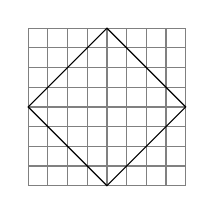
\begin{tikzpicture}
   \draw[step=0.25cm,color=gray] (-1,-1) grid (1,1);
   \draw (1,0) -- (0,1) -- (-1,0) -- (0,-1) -- cycle;
\end{tikzpicture}
\begin{Verbatim}
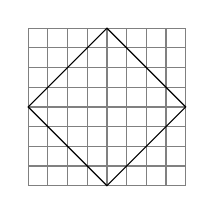
\begin{tikzpicture}
   \draw[step=0.25cm,color=gray] (-1,-1) grid (1,1);
   \draw (1,0) -- (0,1) -- (-1,0) -- (0,-1) -- cycle;
\end{tikzpicture}
\end{Verbatim}
\caption{Zárt vonal ráccsal}
\end{figure}

\begin{figure}
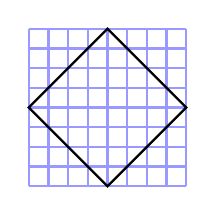
\begin{tikzpicture}[thick]
\definecolor{lightblue}{rgb}{0.600000, 0.600000, 1.000000}
   \draw[step=0.25,color=lightblue] (-1,-1) grid (1,1);
   \draw (1,0) -- (0,1) -- (-1,0) -- (0,-1) -- cycle;
\end{tikzpicture}
\begin{Verbatim}
\definecolor{lightblue}{rgb}{0.600000, 0.600000, 1.000000}
\end{Verbatim}
\caption{Ugyanez kék ráccsal}
\end{figure}

\begin{figure}
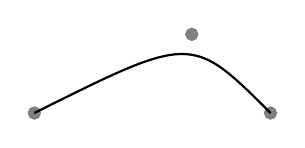
\begin{tikzpicture}[thick]
  \filldraw [gray] (0,0) circle (2pt)
                   (2,1) circle (2pt)
                   (3,0) circle (2pt);
  \draw (0,0) .. controls (2,1) and (2,1) .. (3,0);
\end{tikzpicture}
\begin{Verbatim}
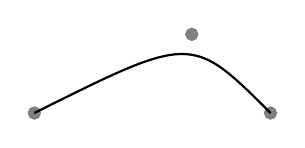
\begin{tikzpicture}[thick]
  \filldraw [gray] (0,0) circle (2pt)
                   (2,1) circle (2pt)
                   (3,0) circle (2pt);
  \draw (0,0) .. controls (2,1) and (2,1) .. (3,0);
\end{tikzpicture}
\end{Verbatim}
\caption{B\`ezier-görbe azonos kontrolponttal}
\end{figure}
%
\begin{figure}
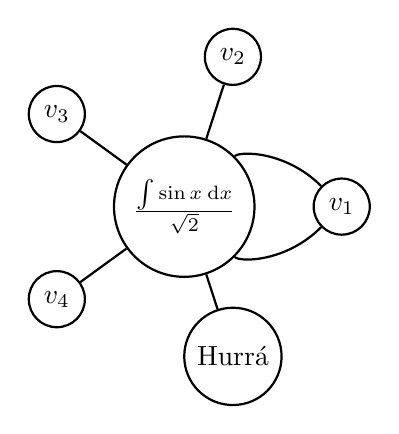
\begin{tikzpicture}[scale=2.0, thick]
   \tikzstyle{every node}=[draw,shape=circle];
   \path (0:0cm)    node (v0) {$\frac{\int \sin x \:\mathrm{d} x}{\sqrt{2}}$};
   \path (0:1cm)    node (v1) {$v_1$};
   \path (72:1cm)   node (v2) {$v_2$};
   \path (2*72:1cm) node (v3) {$v_3$};
   \path (3*72:1cm) node (v4) {$v_4$};
   \path (4*72:1cm) node (v5) {Hurrá};
   \draw (v0) .. controls +(-45:0.5cm) and +(+225:0.5cm) .. (v1)
         (v0) .. controls +(+45:0.5cm) and +(+135:0.5cm) .. (v1)
         (v0) -- (v2)
         (v0) -- (v3)
         (v0) -- (v4)
         (v0) -- (v5);
\end{tikzpicture}
\begin{Verbatim}
   \tikzstyle{every node}=[draw,shape=circle];
   \path (0:0cm)    node (v0) {$\int v_0$};
   \path (0:1cm)    node (v1) {$v_1$};
   \path (72:1cm)   node (v2) {$v_2$};
   \path (2*72:1cm) node (v3) {$v_3$};
   \path (3*72:1cm) node (v4) {$v_4$};
   \path (4*72:1cm) node (v5) {Hurrá};
   \draw (v0) .. controls +(-45:0.5cm) and +(+225:0.5cm) .. (v1)
         (v0) .. controls +(+45:0.5cm) and +(+135:0.5cm) .. (v1)
         (v0) -- (v2)
         (v0) -- (v3)
         (v0) -- (v4)
         (v0) -- (v5);
\end{Verbatim}
\caption{Multigráf B\`ezier-görbével}
\end{figure}

\begin{figure}
% Graphic for TeX using PGF
% Title: /home/ha/ec/fig/fizika/kocsi.dia
% Creator: Dia v0.96.1
% CreationDate: Mon May 18 13:18:35 2009
% For: ha
% \usepackage{tikz}
% The following commands are not supported in PSTricks at present
% We define them conditionally, so when they are implemented,
% this pgf file will use them.
\ifx\du\undefined
  \newlength{\du}
\fi
\setlength{\du}{10\unitlength}
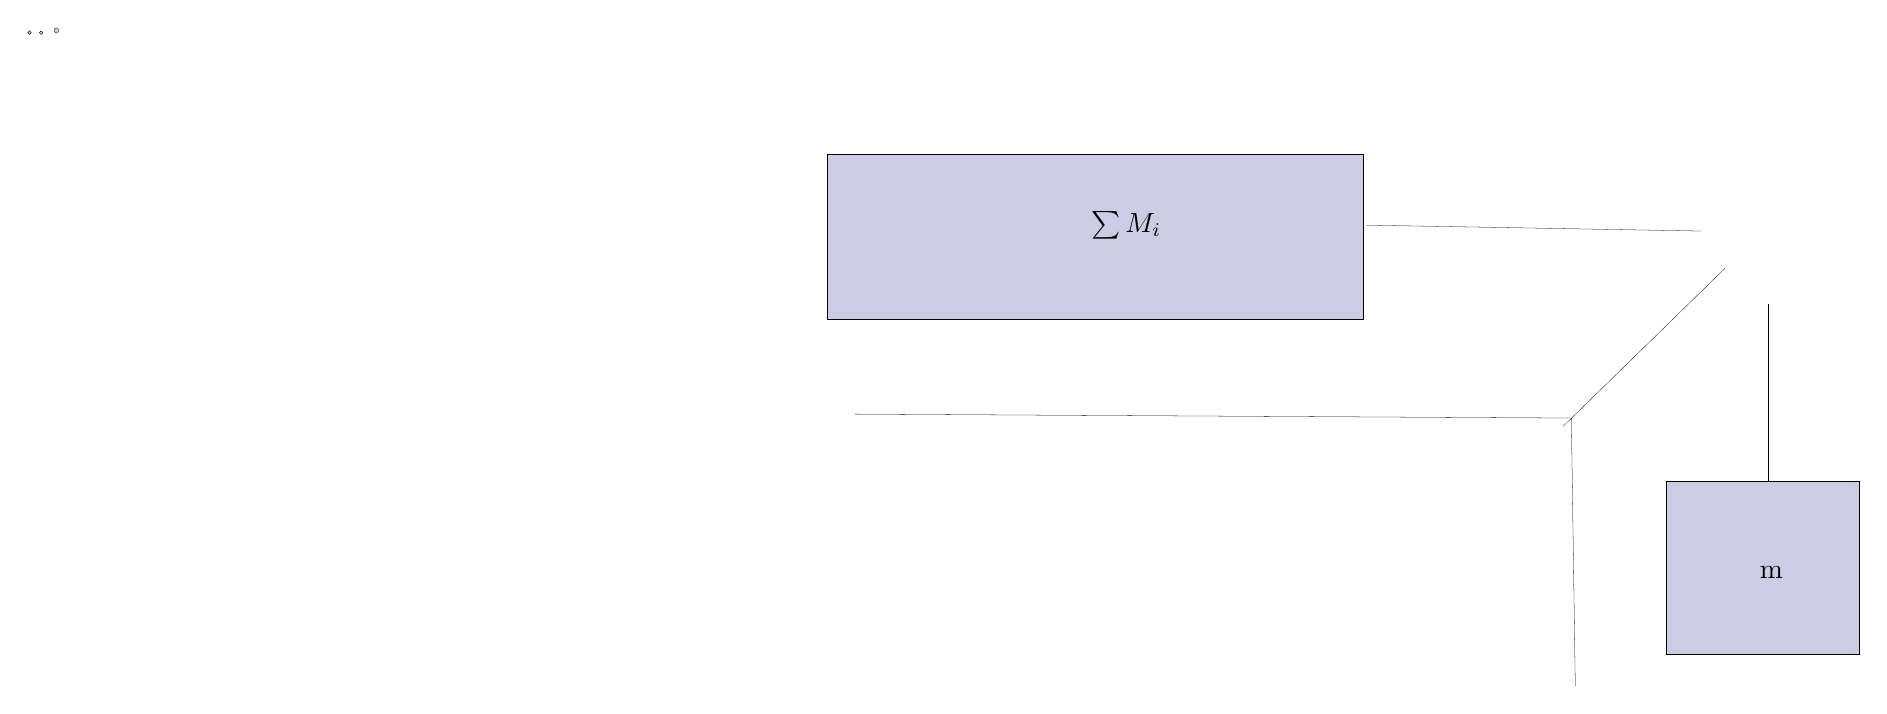
\begin{tikzpicture}
\pgftransformxscale{1.000000}
\pgftransformyscale{-1.000000}
\definecolor{fillcolor}{rgb}{0.8, 0.8, 0.9}
\pgfsetfillcolor{fillcolor}
\pgfsetlinewidth{0.100000\du}
\pgfsetdash{}{0pt}
\pgfsetdash{}{0pt}
\pgfsetmiterjoin
\pgfsetbuttcap
{\pgfsetcornersarced{\pgfpoint{0.000000\du}{0.000000\du}}\definecolor{dialinecolor}{rgb}{0.000000, 0.000000, 0.000000}
\pgfsetstrokecolor{dialinecolor}
\draw (10.900000\du,5.000000\du)--(20.000000\du,5.050000\du)--(20.050000\du,8.450000\du);
}
\pgfsetlinewidth{0.100000\du}
\pgfsetdash{}{0pt}
\pgfsetdash{}{0pt}
\pgfsetbuttcap
\pgfsetmiterjoin
\pgfsetlinewidth{0.100000\du}
\pgfsetbuttcap
\pgfsetmiterjoin
\pgfsetdash{}{0pt}
\pgfpathellipse{\pgfpoint{11.937500\du}{4.387500\du}}{\pgfpoint{0.637500\du}{0\du}}{\pgfpoint{0\du}{0.637500\du}}
\pgfusepath{fill}
\pgfpathellipse{\pgfpoint{11.937500\du}{4.387500\du}}{\pgfpoint{0.637500\du}{0\du}}{\pgfpoint{0\du}{0.637500\du}}
\pgfusepath{stroke}
\pgfsetlinewidth{0.010000\du}
\pgfsetbuttcap
\pgfsetmiterjoin
\pgfsetdash{}{0pt}
\pgfpathellipse{\pgfpoint{11.937500\du}{4.387500\du}}{\pgfpoint{0.637500\du}{0\du}}{\pgfpoint{0\du}{0.637500\du}}
\pgfusepath{stroke}
\pgfsetlinewidth{0.100000\du}
\pgfsetdash{}{0pt}
\pgfsetdash{}{0pt}
\pgfsetbuttcap
\pgfsetmiterjoin
\pgfsetlinewidth{0.100000\du}
\pgfsetbuttcap
\pgfsetmiterjoin
\pgfsetdash{}{0pt}
\pgfpathellipse{\pgfpoint{16.122500\du}{4.432500\du}}{\pgfpoint{0.637500\du}{0\du}}{\pgfpoint{0\du}{0.637500\du}}
\pgfusepath{fill}
\pgfpathellipse{\pgfpoint{16.122500\du}{4.432500\du}}{\pgfpoint{0.637500\du}{0\du}}{\pgfpoint{0\du}{0.637500\du}}
\pgfusepath{stroke}
\pgfsetlinewidth{0.010000\du}
\pgfsetbuttcap
\pgfsetmiterjoin
\pgfsetdash{}{0pt}
\pgfpathellipse{\pgfpoint{16.122500\du}{4.432500\du}}{\pgfpoint{0.637500\du}{0\du}}{\pgfpoint{0\du}{0.637500\du}}
\pgfusepath{stroke}
\pgfsetlinewidth{0.100000\du}
\pgfsetdash{}{0pt}
\pgfsetdash{}{0pt}
\pgfsetmiterjoin
\fill (10.550000\du,1.700000\du)--(10.550000\du,3.800000\du)--(17.350000\du,3.800000\du)--(17.350000\du,1.700000\du)--cycle;
\draw (10.550000\du,1.700000\du)--(10.550000\du,3.800000\du)--(17.350000\du,3.800000\du)--(17.350000\du,1.700000\du)--cycle;
\pgfsetlinewidth{0.100000\du}
\pgfsetdash{}{0pt}
\pgfsetdash{}{0pt}
\pgfsetbuttcap
{
\draw (19.900000\du,5.150000\du)--(21.950000\du,3.150000\du);
}
\pgfpathellipse{\pgfpoint{21.650000\du}{3.600000\du}}{\pgfpoint{0.850000\du}{0\du}}{\pgfpoint{0\du}{0.925000\du}}
\pgfusepath{fill}
\pgfsetlinewidth{0.100000\du}
\pgfsetdash{}{0pt}
\pgfsetdash{}{0pt}
\pgfpathellipse{\pgfpoint{21.650000\du}{3.600000\du}}{\pgfpoint{0.850000\du}{0\du}}{\pgfpoint{0\du}{0.925000\du}}
\pgfusepath{stroke}
\pgfsetlinewidth{0.100000\du}
\pgfsetdash{}{0pt}
\pgfsetdash{}{0pt}
\pgfsetbuttcap
{
\definecolor{dialinecolor}{rgb}{0.000000, 0.000000, 0.000000}
\pgfsetstrokecolor{dialinecolor}
\draw (17.4000000\du,2.600000\du)--(21.650000\du,2.675000\du);
}
\pgfsetlinewidth{0.100000\du}
\pgfsetdash{}{0pt}
\pgfsetdash{}{0pt}
\pgfsetbuttcap
{
\definecolor{dialinecolor}{rgb}{0.000000, 0.000000, 0.000000}
\pgfsetfillcolor{dialinecolor}
% was here!!!
\definecolor{dialinecolor}{rgb}{0.000000, 0.000000, 0.000000}
\pgfsetstrokecolor{dialinecolor}
\draw (22.500000\du,3.600000\du)--(22.500000\du,8.050000\du);
}
\pgfsetlinewidth{0.100000\du}
\pgfsetdash{}{0pt}
\pgfsetdash{}{0pt}
\pgfsetmiterjoin
\definecolor{dialinecolor}{rgb}{000000, 1.000000, 1.000000}
\pgfsetfillcolor{fillcolor}
\fill (21.200000\du,5.850000\du)--(21.200000\du,8.050000\du)--(23.650000\du,8.050000\du)--(23.650000\du,5.850000\du)--cycle;
\definecolor{dialinecolor}{rgb}{0.000000, 0.000000, 0.000000}
\pgfsetstrokecolor{dialinecolor}
\draw (21.200000\du,5.850000\du)--(21.200000\du,8.050000\du)--(23.650000\du,8.050000\du)--(23.650000\du,5.850000\du)--cycle;
% setfont left to latex
\definecolor{dialinecolor}{rgb}{0.000000, 0.000000, 0.000000}
\pgfsetstrokecolor{dialinecolor}
\node at (14.350000\du,2.600000\du){$\sum M_i$};
% setfont left to latex
\definecolor{dialinecolor}{rgb}{0.000000, 0.000000, 0.000000}
\pgfsetstrokecolor{dialinecolor}
\node at (22.541250\du,7.013969\du){m};
\end{tikzpicture}
\caption{Kiskocsi, amelyet a Dia rajzolóprogrammal csináltam.}
\end{figure}

\begin{figure}
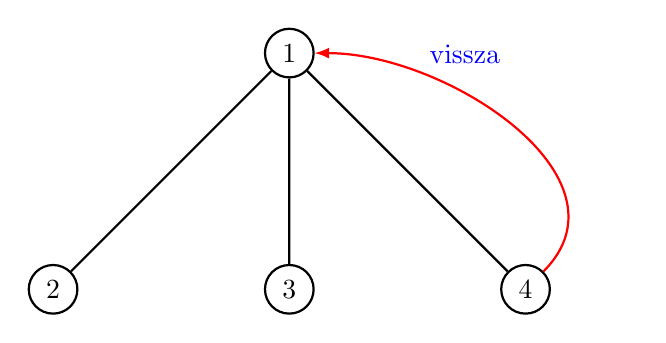
\begin{tikzpicture}[scale=2, thick]
    \tikzstyle{every node}=[draw,circle]

    \node (root) {1}
        child { node {2} }
        child { node {3} }
        child { node (rightmost) {4} }
    ;

    \tikzstyle{every node}=[]

    \draw[-latex,color=red]
        (rightmost) .. controls +(45:1) and
                                +(0:1) ..
            node[near end,above right,color=blue] {vissza}
        (root);
\end{tikzpicture}
\caption{Fát is rajzolhatunk vele.}
\end{figure}

\begin{figure}
\usetikzlibrary{positioning}
\large
\begin{tikzpicture}[every node/.style={minimum size=1cm},on grid]
\begin{scope}[every node/.append style={yslant=-0.5},yslant=-0.5]
  \shade[right color=gray!10, left color=black!50] (0,0) rectangle +(3,3);
  \node at (0.5,2.5) {9};
  \node at (1.5,2.5) {7};
  \node at (2.5,2.5) {1};
  \node at (0.5,1.5) {2};
  \node at (1.5,1.5) {4};
  \node at (2.5,1.5) {8};
  \node at (0.5,0.5) {5};
  \node at (1.5,0.5) {3};
  \node at (2.5,0.5) {6};
  \draw (0,0) grid (3,3);
\end{scope}
\begin{scope}[every node/.append style={yslant=0.5},yslant=0.5]
  \shade[right color=gray!70,left color=gray!10] (3,-3) rectangle +(3,3);
  \node at (3.5,-0.5) {3};
  \node at (4.5,-0.5) {9};
  \node at (5.5,-0.5) {7};
  \node at (3.5,-1.5) {6};
  \node at (4.5,-1.5) {1};
  \node at (5.5,-1.5) {5};
  \node at (3.5,-2.5) {8};
  \node at (4.5,-2.5) {2};
  \node at (5.5,-2.5) {4};
  \draw (3,-3) grid (6,0);
\end{scope}
\begin{scope}[every node/.append style={yslant=0.5,xslant=-1},yslant=0.5,xslant=-1]
  \shade[bottom color=gray!10, top color=black!80] (6,3) rectangle +(-3,-3);
  \node at (3.5,2.5) {1};
  \node at (3.5,1.5) {4};
  \node at (3.5,0.5) {7};
  \node at (4.5,2.5) {5};
  \node at (4.5,1.5) {6};
  \node at (4.5,0.5) {8};
  \node at (5.5,2.5) {2};
  \node at (5.5,1.5) {3};
  \node at (5.5,0.5) {9};
  \draw (3,0) grid (6,3);
\end{scope}
\end{tikzpicture}
\caption{Ez szép, de csak bemásoltam.}
\end{figure}

\begin{figure}
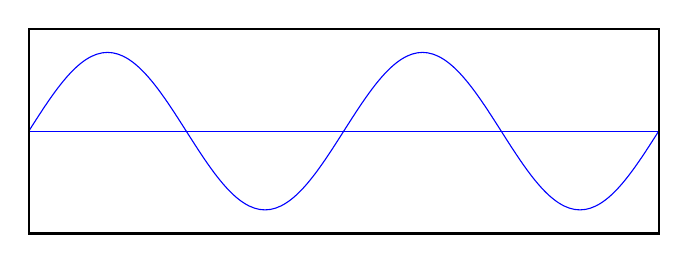
\begin{tikzpicture}%[x=10pt, y=5pt]
 \draw[color=blue] (0,0) sin ++(1,1) cos ++(1,-1) sin ++(1,-1) cos ++(1,1)
 sin ++(1,1) cos ++(1,-1) sin ++(1,-1) cos ++(1,1);
 \draw[color=blue] (0,0) -- (8,0);
 %\draw (0,-1) rectangle (8,1);
 \draw[thick] (0,-1.3) rectangle (8,1.3);
\end{tikzpicture}
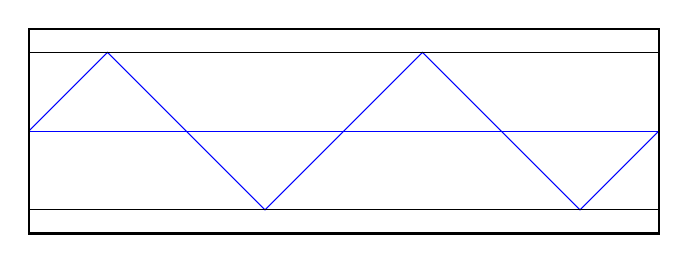
\begin{tikzpicture}%[x=10pt, y=5pt]
 \draw[color=blue] (0,0) -- ++(1,1) -- ++(1,-1) -- ++(1,-1) -- ++(1,1)
 -- ++(1,1) -- ++(1,-1) -- ++(1,-1) -- ++(1,1);
 \draw[color=blue] (0,0) -- (8,0);
 \draw (0,-1) rectangle (8,1);
 \draw[thick] (0,-1.3) rectangle (8,1.3);
\end{tikzpicture}
\caption{A parabolikus profilú (GRIN=GRaded INdex) és a lépcsős profilú
szál két jellemző sugármenete. A GRIN szálban a hosszabb úton haladó
sugár átlagosan gyorsabban megy, így a késése kisebb, mint a lépcsős
profilúnál, tehát egy beérkező fényimpulzus esetén, amelyből mindkét
irányban jut fénysugár, kisebb lesz a szál túlsó végén az impulzus
,,szétfolyása''.}
\end{figure}

\begin{figure}
\caption{Lépcsős profilú}
\end{figure}

\end{document}
